% !TEX root = ../thesis.tex

\section{Dataset and Preprocessing}
\label{sec:method:data}

\subsection{The Diabetes 130-US Hospitals Dataset}
\label{sec:data:dataset}

The dataset used throughout this thesis is the \emph{UCI Diabetes 130-US
Hospitals} dataset~\cite{diabetes_db,strack2014impact}. It contains 101{,}766
inpatient encounters from diabetic patients treated across 130 U.S.\ hospitals
between 1999 and 2008. Each record describes a hospital admission of 1-14
days and includes 50 columns: mixed-type features covering demographics (age,
gender, race), admission characteristics, laboratory test results, diagnoses,
medication use, and prior inpatient, outpatient, and emergency visits,
together with record identifiers and the readmission target. The
data consists primarily of categorical and integer variables and represents
detailed clinical, administrative, and treatment-related information collected
during the patient's hospital stay. 

This dataset was selected because it provides a large, publicly available,
real-world medical benchmark with a clinically meaningful readmission outcome,
while still remaining computationally manageable for repeated generator
training and evaluation. Its relevance is further supported by prior synthetic
health-data work using HealthGAN-style privacy and utility evaluation
protocols~\cite{healthgan}.

Missing values are present, and no
predefined data splits are provided. This enables flexible
train-validation-test partitioning. The binary target used throughout this
work is \emph{readmitted}. Hospital readmissions of any kind are encoded as
the positive class and ``no readmission'' as the negative class.

\paragraph{Scope:} The proposal contemplated MIMIC-III as a secondary
benchmark; the final thesis is restricted to the Diabetes 130-US Hospitals
dataset to keep training budgets and evaluation runs manageable across five
generators and twelve single-number metrics. Cross-dataset generalisation is discussed as
future work in Section~\ref{sec:conclusion:future}.

\subsection{Exploratory Data Analysis}
\label{sec:data:eda}

An exploratory analysis of the raw dataset is conducted to characterise its
schema, missingness structure, feature imbalance, and target distribution.
The observations summarised below motivate the engineering choices
described in Section~\ref{sec:data:fe}.

\paragraph{Schema and missingness:}
The raw CSV contains 50 columns: 10 integer columns and 40 categorical columns.
The integer fields include encounter and patient identifiers, procedure,
medication and diagnosis counts, and length of stay. Most remaining
fields are categorical, including demographic variables, admission and
discharge codes, ICD-9 diagnosis codes, laboratory-result indicators,
medication-change indicators, and the readmission target. The token
\emph{?} is treated as a missing value, and known count and identifier
fields are cast to numeric type while the remaining columns are retained
as categorical variables. Missingness is concentrated in a small number of
clinical and administrative fields, five of which exceed $39\%$ absent:
\emph{weight} ($96.86\%$), \emph{max\_glu\_serum} ($94.75\%$),
\emph{A1Cresult} ($83.28\%$), \emph{medical\_specialty} ($49.08\%$), and
\emph{payer\_code} ($39.56\%$). The remaining columns are near-complete, with
the full breakdown shown in Figure~\ref{fig:data:missingness}. The engineering
response to these patterns (field removal versus imputation) is described in
Section~\ref{sec:data:fe}.

\begin{figure}[h]
\centering
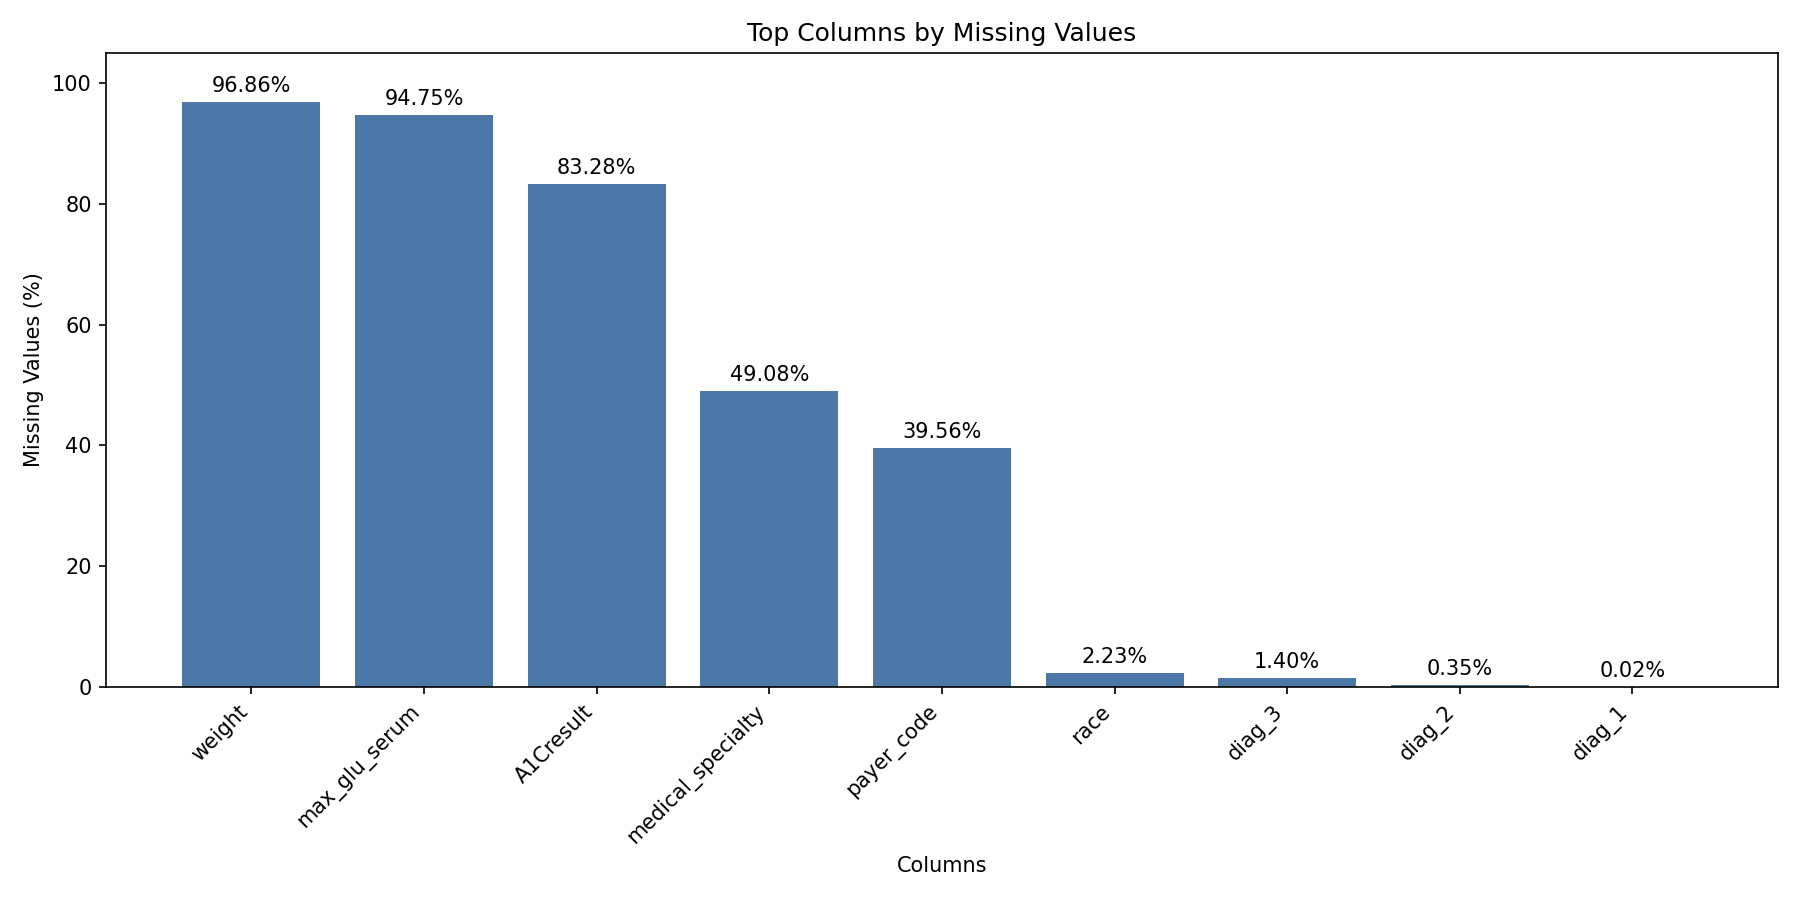
\includegraphics[width=0.95\textwidth]{images/data/missingness}
\caption{Proportion of missing values in the raw dataset.}
\label{fig:data:missingness}
\end{figure}

\paragraph{Medication imbalance:}
Fifteen of the twenty-three medication fields in the raw dataset exhibit 
severe class imbalance. In each of these fields, the dominant value 
\emph{No} accounts for more than 99\% of encounters. This leaves fewer than 
1\% non-modal observations. Among the affected fields are rare agents such as
\emph{examide}, \emph{citoglipton}, \emph{troglitazone}, and several
combination medications. Highly imbalanced categorical columns are a known challenge for tabular GANs
and can lead to mode collapse or missing minor categories~\cite{Xu2019CTGAN}. The corresponding encoding
transformation applied to these fields is described in
Section~\ref{sec:data:fe}.

\paragraph{Target distribution:}
The raw target has three categories: \emph{NO}, \emph{>30}, and
\emph{<30}. In the full raw dataset, \emph{NO} accounts for 54{,}864
encounters (53.91\%), \emph{>30} for 35{,}545 encounters (34.93\%), and
\emph{<30} for 11{,}357 encounters (11.16\%). The two readmission
categories are collapsed into a single positive class in
Section~\ref{sec:data:fe}, reducing the prediction task to binary
readmission. After multiple-encounter resolution and target binarisation,
the processed dataset contains 47{,}188 non-readmitted records (65.98\%)
and 24{,}330 readmitted records (34.02\%). The stratified training split
preserves this imbalance with 37{,}750 negatives and 19{,}464 positives.
This class distribution defines a baseline marginal that any synthetic
generator is required to preserve; deviation is quantified in
Section~\ref{sec:results:rq2:utility:similarity}.

\paragraph{Summary:}
Together, these properties define the design constraints addressed by 
the engineering pipeline of Section~\ref{sec:data:fe}. These properties 
include high missingness in a small set of administrative fields, severe 
imbalance in rare-medication indicators, and a multi-class readmission 
target requiring binary collapse.

\subsection{Feature Engineering}
\label{sec:data:fe}

The engineering pipeline performs eight transformations in fixed order:
(1)~multi-encounter resolution, (2)~age encoding, (3)~field removal,
(4)~diagnosis grouping, (5)~medication binarisation, (6)~A1C ordinal
encoding, (7)~imputation and label encoding, and (8)~target binarisation.
Row-level deduplication and clinically motivated grouping precede
imputation and label encoding so that each downstream step sees a clean,
deduplicated input.

\paragraph{Multi-encounter resolution and identifier removal:}
The raw dataset contains repeated encounters for some patients: although
there are 101{,}766 encounter rows, there are 71{,}518 unique values of
\emph{patient\_nbr}; 16{,}773 patients appear more than once, and the
maximum number of encounters for a single patient is 40. To avoid
patient-level leakage between train and test splits, multi-encounter rows
are resolved by sorting on
\emph{patient\_nbr} and \emph{time\_in\_hospital}, retaining the
encounter with the longest hospital stay, and dropping duplicate patient
rows. \emph{patient\_nbr} is then removed as a direct patient identifier,
and \emph{race} is removed to limit reliance on a sensitive demographic
field.

\paragraph{Age encoding:}
\label{sec:data:fe:age}%
The decade-based age buckets are converted to ordered numeric values where
\path{[0-10)} maps to 1, \path{[10-20)}
to 2, and so on through \emph{[90-100)}, which maps to 10. The 1-10
ordinal encoding preserves the natural ordering of age while avoiding a
high-cardinality categorical representation. An earlier preprocessing
variant collapsed the ten decades into a three-level grouping
(young / middle-aged / elderly) to reduce categorical sparsity. A direct
ablation against the ten-bin encoding informed the final choice.
The ten-bin encoding is retained for all experiments in this thesis, and
the quantitative comparison is deferred to
Section~\ref{sec:results:rq2:utility:age-binning}.

\paragraph{Field removal:}
Three high-missingness fields: \emph{weight} (96.86\%),
\emph{payer\_code} (39.56\%), and \emph{medical\_specialty} (49.08\%)
are dropped to reduce dimensionality and to limit the parameter
capacity that synthetic-data generators must allocate to sparsely
observed features. Although \emph{A1Cresult} and \emph{max\_glu\_serum} 
also exceed 80\% missingness, they are retained because their
absence can be represented as an explicit ``not measured'' category rather than
as an unknown continuous value.

\paragraph{Diagnosis grouping:}
The three diagnosis fields \emph{diag\_1}, \emph{diag\_2}, and
\emph{diag\_3} together contain 915 distinct ICD-9 codes in the raw
dataset. These are mapped to broader diagnosis groups: codes
beginning with 250 are mapped to \emph{Diabetes}, and numeric ICD-9
ranges are grouped as circulatory, respiratory, digestive, genitourinary,
neoplasm, musculoskeletal, and injury categories. External cause and
supplementary codes beginning with \emph{E} or \emph{V}, missing
values, and unrecognised codes are mapped to \emph{Other}. The grouping
is a clinically motivated taxonomy inspired by Strack et
al.~\cite{strack2014impact} and is not derived from the standard Clinical
Classifications Software (CCS) / Healthcare Cost and Utilization Project 
(HCUP) mapping. The step reduces the 915-code ICD-9 vocabulary into nine
clinically interpretable categories, which are converted to integer
labels later by the label-encoding step.

\paragraph{Medication binarisation:}
The 23 medication columns are converted to binary exposure indicators: \emph{No} is encoded as 0, and
every other observed value (including \emph{Steady}, \emph{Up}, and
\emph{Down}) is encoded as 1. The binary representation records whether
a medication was prescribed or changed during the encounter, rather than
modelling the rare dosage-direction levels as separate categories. This
mitigates the severe medication imbalance documented in
Section~\ref{sec:data:eda}.

\paragraph{A1C ordinal encoding:}
The \emph{A1Cresult} field is converted to an ordinal laboratory
indicator. Missing A1C values are encoded as
0, with the remaining levels mapped as \emph{Norm}~$\rightarrow$~1,
\emph{>7}~$\rightarrow$~2, and \emph{>8}~$\rightarrow$~3. The 0 level
retains the absence of an A1C test as an explicit category while
preserving the ordinal severity of observed results.

\paragraph{Imputation and label encoding:}
Remaining missing values are imputed: categorical
columns by the most frequent observed value and numeric columns by the
median. After imputation, the
preprocessed dataset contains no missing values. All remaining
object-type feature columns are then converted to integer labels,
excluding the target.

\paragraph{Target binarisation:}
The original three-class readmission variable is collapsed to a binary
outcome: \emph{NO} is encoded as 0, while both
\emph{>30} and \emph{<30} are encoded as 1. This any-readmission
formulation is used consistently throughout downstream training and
evaluation.

\paragraph{Feature scaling:}
No additional scaling is applied within the engineering pipeline.
Per-generator normalisation is handled internally by the respective
synthesis frameworks
(Section~\ref{sec:method:generators}).

\subsection{Train/Test Split}
\label{sec:data:split}

Through the preprocessing steps we generate the full preprocessed
dataset (71{,}518 rows, 45 columns), the training split, and the test
split. The split is created with a stratified 80/20 partition
(\emph{test\_size = 0.2}, \emph{random\_state = 42}), with the
target column passed as the stratification variable to preserve the
binary readmission ratio across splits. Because
multi-encounter resolution produces one row per
\emph{patient\_nbr}, the stratified split is inherently patient-disjoint
and free of train-test leakage at the patient level.

The training set contains 57{,}214 rows and 45 columns, with 37{,}750
negative records and 19{,}464 positive records. The held-out test set
contains 14{,}304 rows and 45 columns, with 9{,}438 negative records and
4{,}866 positive records. Both splits contain no missing values and no
object-type columns after preprocessing. The \emph{encounter\_id} column is
retained in the stored splits but excluded from all evaluation.
